\documentclass[14pt]{book}

\usepackage{fancyhdr}
\usepackage{graphicx}
\usepackage[margin=2.5cm]{geometry}
\usepackage{graphicx}
\usepackage{anysize}
\usepackage{xcolor}
\usepackage{caption}
\usepackage{subcaption}

\marginsize{2cm}{2cm}{2cm}{2cm} % Izquierda, derecha, arriba, abajo
\setlength{\parindent}{0cm}
\pagestyle{fancy}
\fancyhf{}
\fancyhead[L]{\footnotesize Redes de computadoras} %encabezado izquierda
\fancyhead[R]{\footnotesize David Pérez Jacome}   % derecha
\fancyfoot[L]{\footnotesize}  %izquierda
\fancyfoot[C]{Página \thepage}
\renewcommand{\footrulewidth}{0.4pt}

\begin{document}
\begin{center}
  \newcommand{\HRule}{\rule{\linewidth}{0.5mm}}
  \begin{minipage}{0.48\textwidth}
    \begin{flushleft}
      
\includegraphics[scale = 0.08]{images/logo_unam.png}
    \end{flushleft}
  \end{minipage}
  \begin{minipage}{0.48\textwidth}
    \begin{flushright}
      
\includegraphics[scale =0.22]{images/logo_ciencias.png}
    \end{flushright}
  \end{minipage}
  \vspace*{-1.5cm}
  \textsc{\huge Nacional Autónoma de México \\ \vspace{-4px} Universidad }\\[2cm]
  \textsc{\LARGE Facultad de Ciencias}\\[1.5cm]
  \begin{minipage}{0.9\textwidth}
    \begin{center}
      \textsc{\LARGE Redes de computadoras}
    \end{center}
  \end{minipage}\\[0.5cm]
  \vspace*{1cm}
  \HRule \\[0.4cm]
  { \huge \bfseries Practica 07}\\[0.4cm]
  \HRule \\[1.5cm]
  \begin{minipage}{0.52\textwidth}
    \begin{flushleft} \large \small \vspace{-0.6cm} \vspace{-0.6cm}
      Alumno David Pérez Jacome \\
    \end{flushleft}
  \end{minipage}
  \begin{minipage}{0.46\textwidth}
    \vspace{-0.6cm}
    \begin{flushright} \large \small \emph{Profesor:}
      Paulo Santiago de Jesús Contreras Flores \\
    \end{flushright}
  \end{minipage}
  \vspace*{1cm}
  \vspace{2cm}
  \begin{center}
    {\large 2023}
  \end{center}
\end{center}
\newpage

{\color{blue} \section*{\textbf{Practica 07}}}
\vspace{1em}

{\color{red} \subsection*{\textbf{Ruteo dinámico con OSPF}}}
\vspace{1em}

{\color{red} \subsection*{\textbf{Objetivo}}}
\vspace{1em}

\begin{enumerate}
  \item El alumno aprenderá el uso del software de simulación de redes Packet Tracer.
  \item Configurará rutas dinámicas usando el protocolo OSPF, en los router de diferentes redes.
  \item Configurará un router para el intercambio de información de rutas entre los protocolos RIP y OSPF.
\end{enumerate}

{\color{red} \subsection*{\textbf{Introducción}}}
\vspace{1em}

El protocolo OSPF (Open Shortest Path First) es un protocolo de ruteo que utiliza el algoritmo de
estado de enlace para la distribución y cálculo de rutas, se desarrolló como reemplazo del protocolo
RIP del tipo vector de distancias. OSPF presenta ventajas importantes en comparación con RIP,
ya que ofrece una convergencia más rápida y un mejor desempeño en redes de mayor tamaño.\\

{\color{red} \subsection*{\textbf{Desarrollo}}}
\vspace{1em}

Desarrollo...

%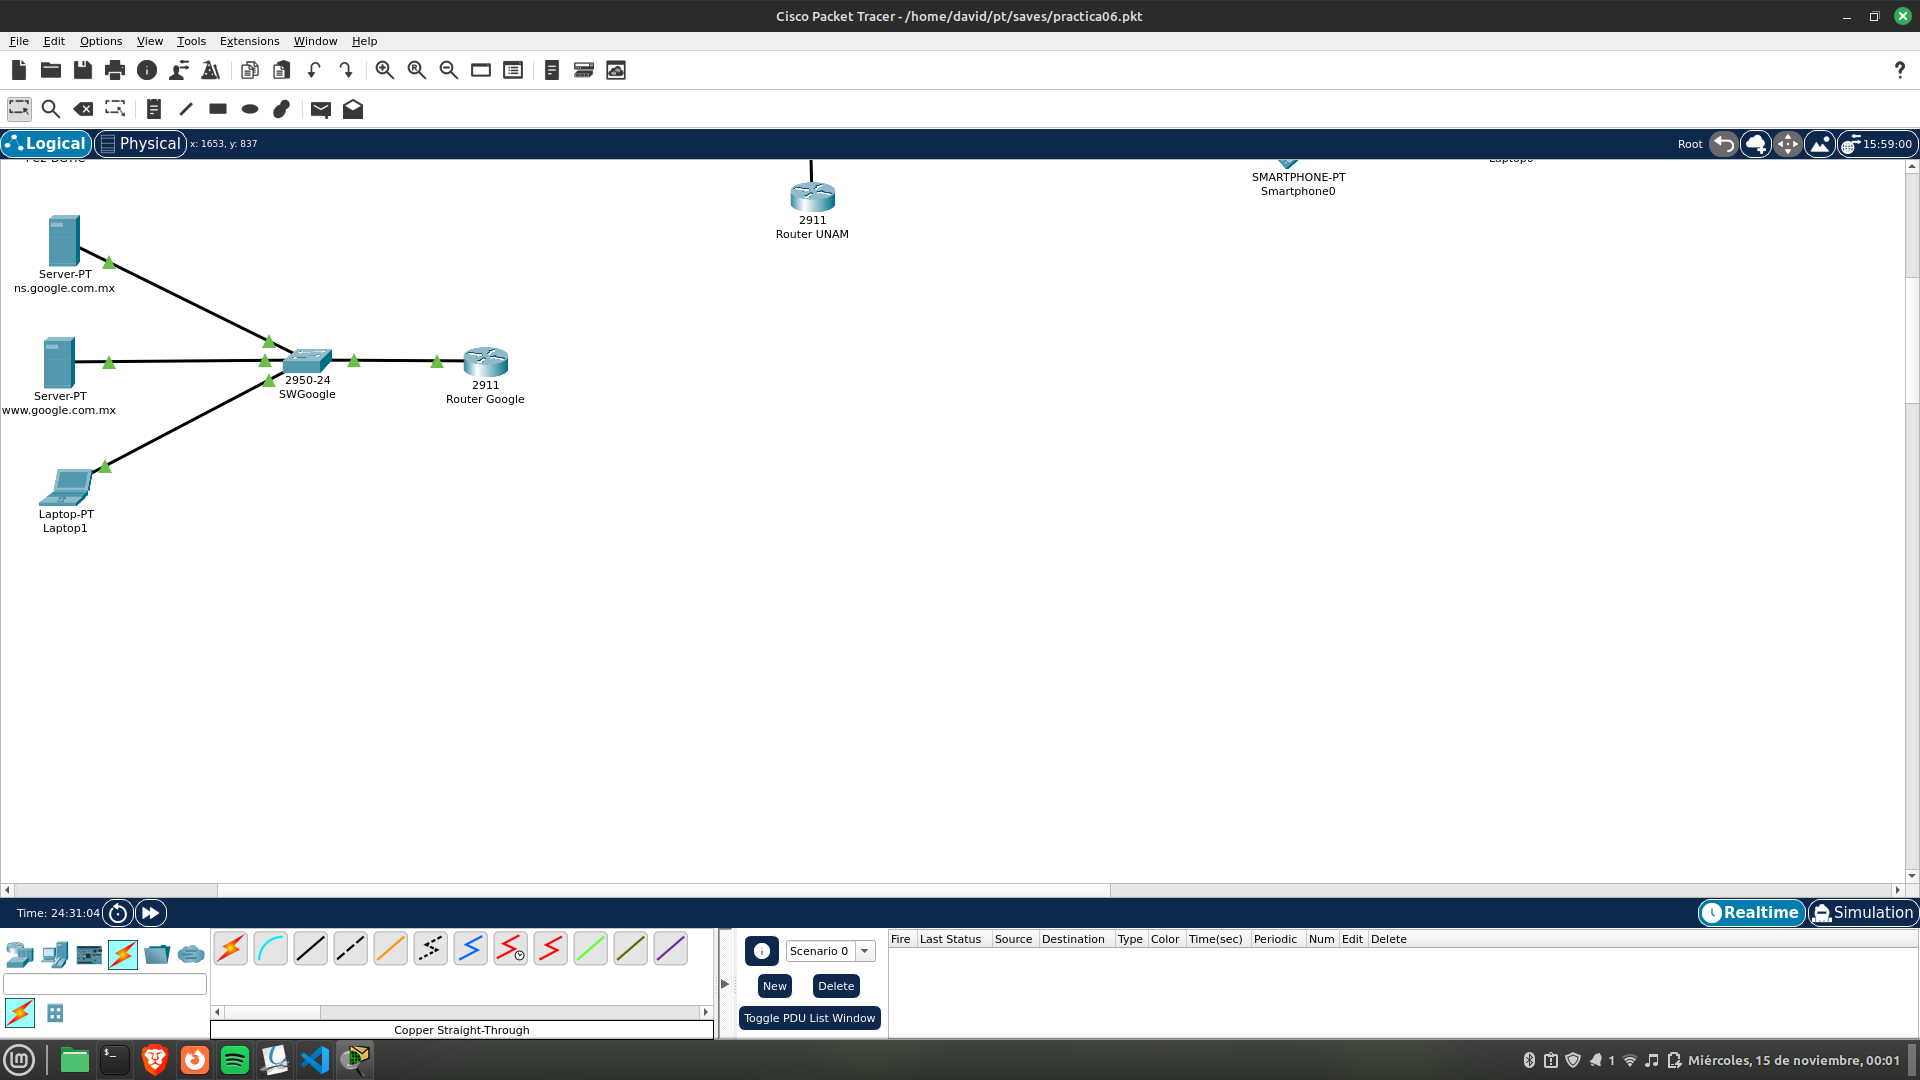
\includegraphics[width=12cm, height=8cm]{images/redgoogle.png}\\

 

\end{document}